%--------------------------------------------------------------------------------
%
%
%--------------------------------------------------------------------------------
\chapter*{Simulator Windows}
\addcontentsline{toc}{chapter}{Simulator Windows}

At the heart of the simulator is the concept of a window to show and modify the simulation environment.
 
%-------------------------------------------------------------------------------- 
\section*{Window Concepts}
\addcontentsline{toc}{section}{Window Concepts}

A window consists of a \textbf{window banner line} and a \textbf{window body}. The banner line begins with the window identification, which includes the window stack number and the window number. The window number is a unique identifier that can be used to refer to a specific window. Beneath the window banner line is the window body, which consists of several lines of ascii text. Both areas are window types specific and display status information, messages and simulator output. 

\begin{figure}[H]
\centering
\begin{tikzpicture}[x=1cm, y=1cm, scale=0.7, transform shape]

    \draw[help lines, gray!70, dashed] (0,0) grid (16,16);

    % Image
    \node[anchor=south west] (img) at (0, 0)
        {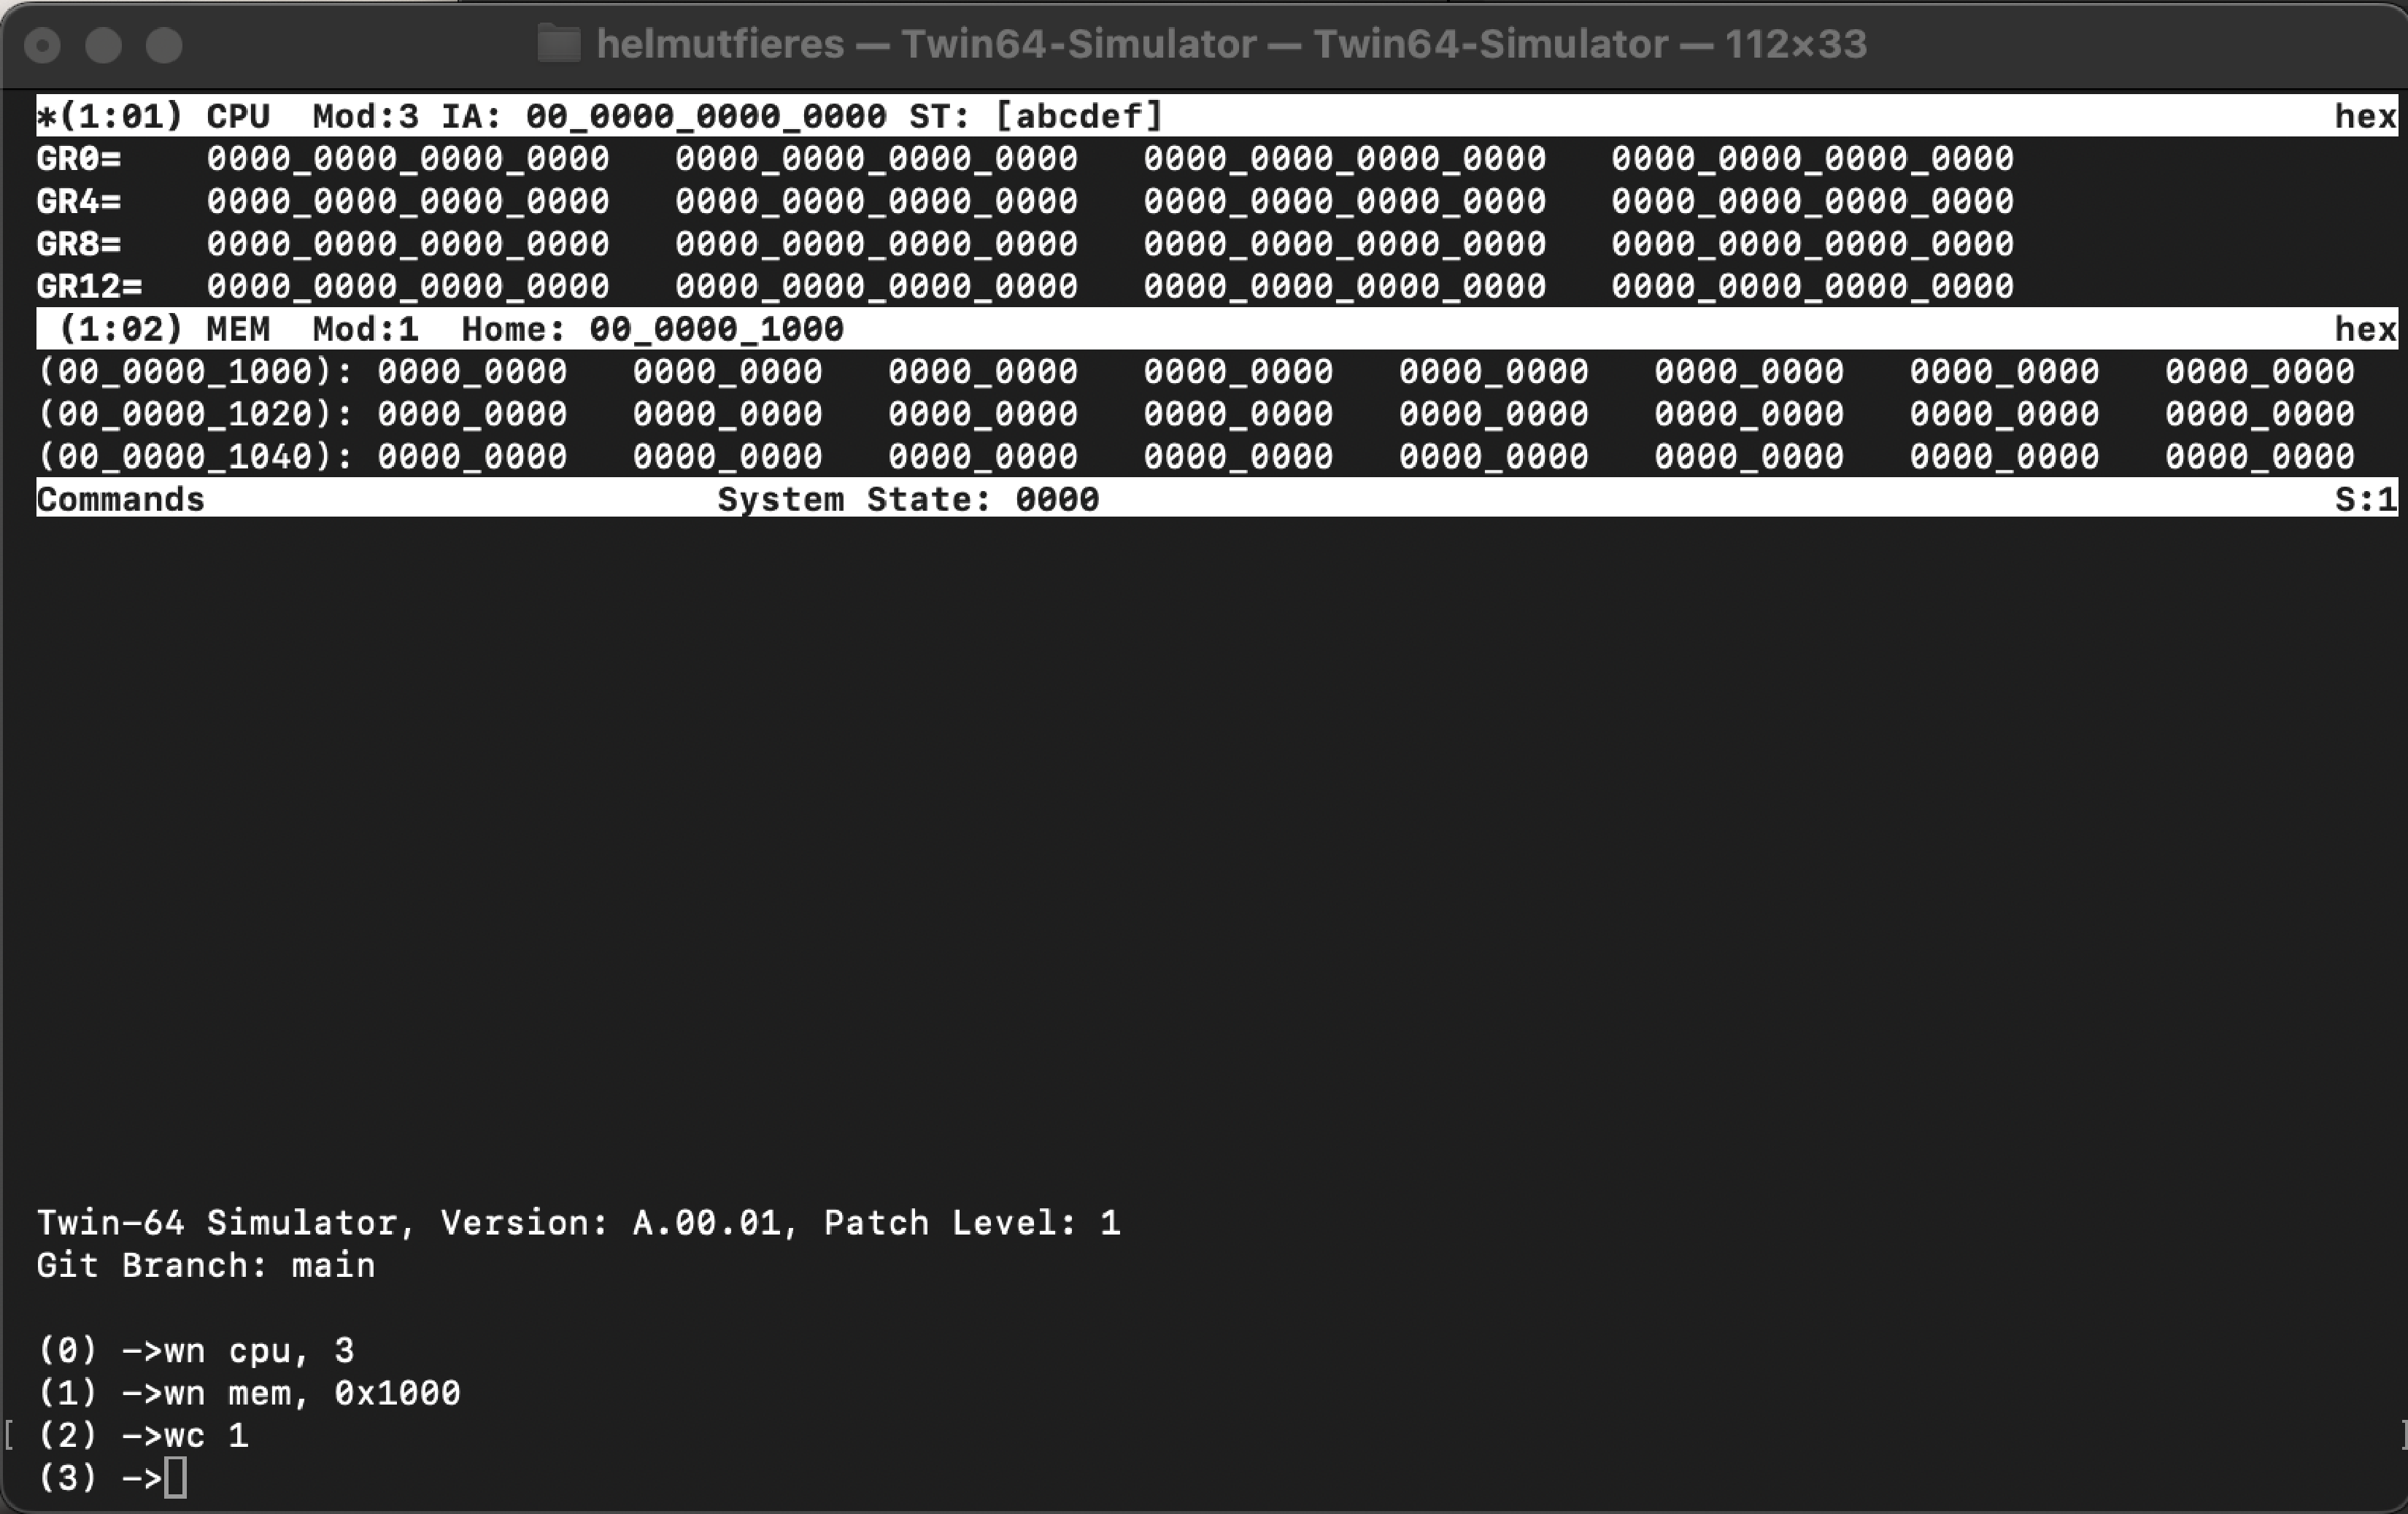
\includegraphics[width=16cm]{chapter-simulator-environment/SimWindows.pdf}};

    % Arrows
    \draw[gray, thick] (0.6, 13.25) -- (1.2, 16);
    \node[anchor=west] at ( 1.25, 16 ) {\Large Window is Current};
    
    \draw[gray, thick] (0.9, 13.25) -- (2.25, 15.25);
    \node[anchor=west] at ( 2.25, 15.25 ) {\Large Window Stack Number};
    
    \draw[gray, thick] (1.25, 13.25) -- (3.25, 14.5);
    \node[anchor=west] at ( 3.25, 14.5 ) {\Large Window Number};
    
    \draw[gray, thick] (9.2, 13.1) -- (11.25, 15.25);
    \node[anchor=west] at ( 11.25, 15.25 ) {\LARGE Window Banner};
    
    \draw[gray, thick] (10, 10.75) -- (12.25, 14.5);
    \node[anchor=west] at ( 12.25, 14.5 ) {\LARGE Window Body};
    
\end{tikzpicture}
\caption{Simulator Windows}
\label{fig:simulator-windows}
\end{figure}

Windows can be organized into stacks. This allows related windows—for example, all windows associated with a single CPU—to be grouped together. A stack can be displayed or hidden as a whole. At all times, exactly one window is designated as the current window. The current window is marked with a star (*) symbol in the banner line. If a window command does not explicitly specify a window identifier, it operates on the current window.

The remainder of the banner line is specific to the window type and is described in the following sections of this manual. At the right edge of the banner line, each window displays the radix format used for presenting its data. The command window banner line displays the currently defined window stacks at the right edge.

%--------------------------------------------------------------------------------
\section*{Window Stacks}
\addcontentsline{toc}{section}{Window Stacks}

Simulator windows can be organized into \textbf{window stacks}. All visible stacks are displayed horizontally with the terminal screen size adjusted accordingly. The following figure shows a two stack example.

\begin{figure}[H]
\centering
\begin{tikzpicture}[x=1cm, y=1cm, scale=0.7, transform shape]
    \node[anchor=south west] (img) at (0, 0)
        {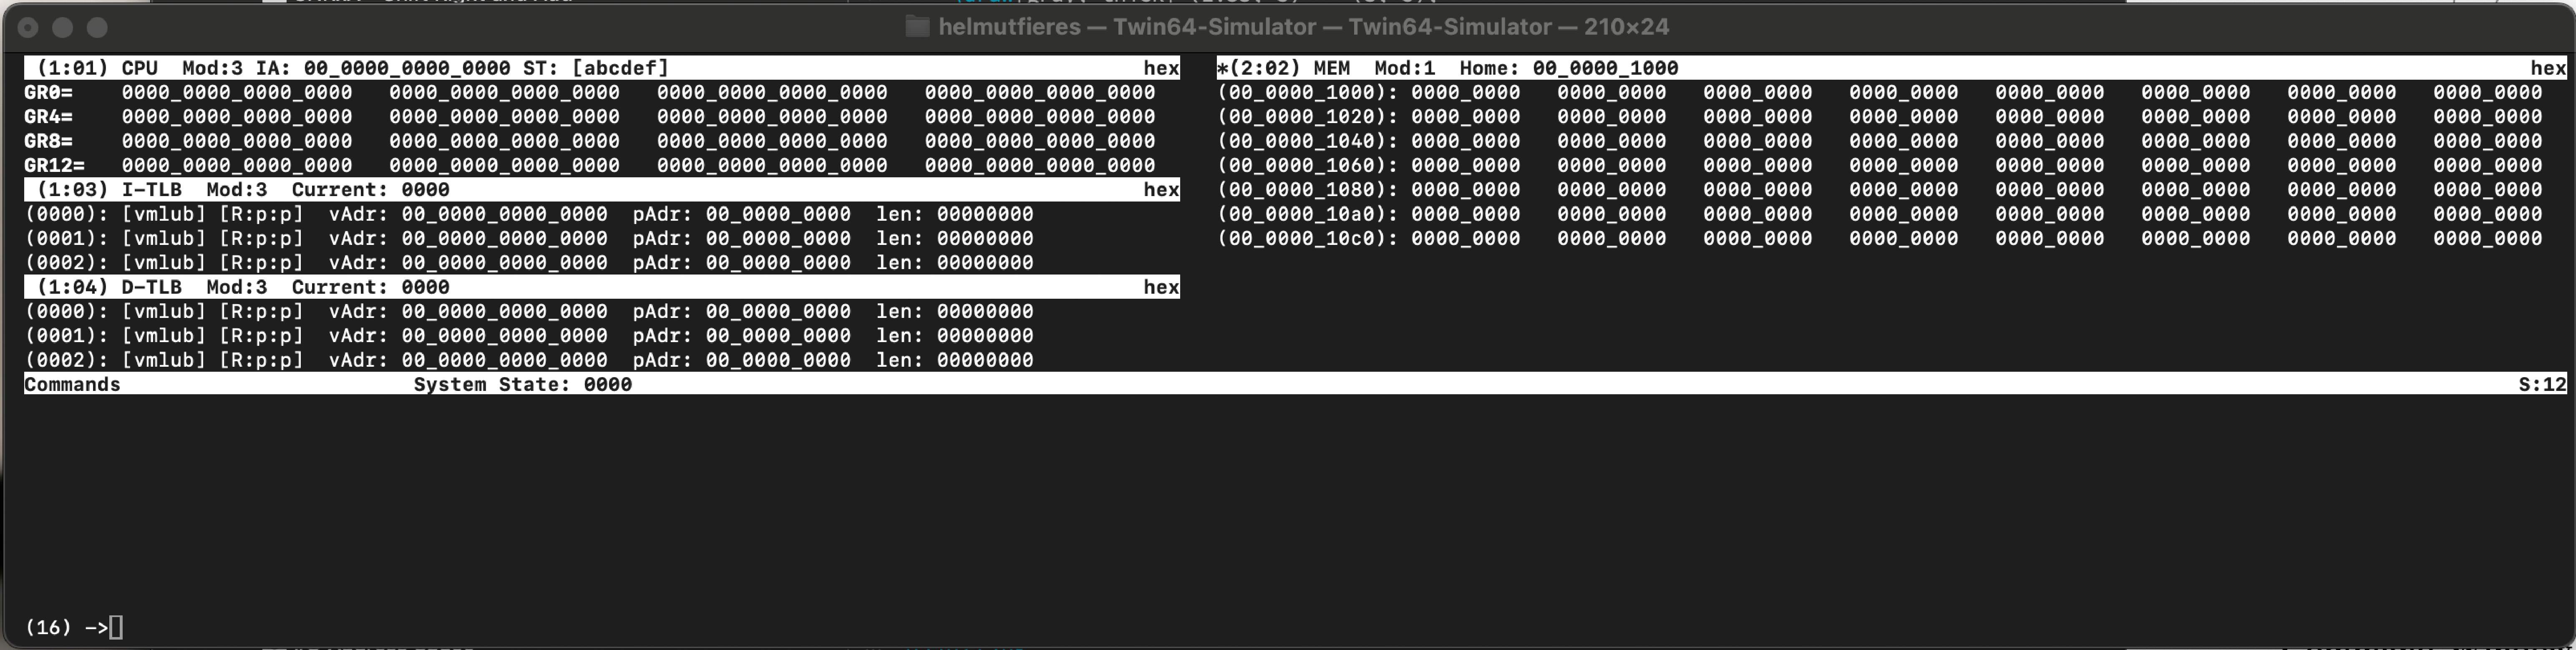
\includegraphics[width=16cm]{chapter-simulator-environment/SimWinStacks.pdf}};
\end{tikzpicture}
\caption{Simulator Window Stacks}
\label{fig:simulator-window-stacks}
\end{figure}

Window stack are very useful when handling several processors and memory content. For example, all windows related to a processor can be grouped in a stack. Windows in a stack can be sorted and individual windows can be enabled or disabled. Disabled windows, like disabled stacks, do not disappear for the overall window list. They are just not displayed.

Naturally, a monitor screen cannot display more than two or three stacks next to each other. Stacks, like windows, can therefore be disabled. A disabled stack is not shown. The command window has a little status filed in its banner line which shows what stacks have been created. 

%--------------------------------------------------------------------------------
\section*{Processor Window}
\addcontentsline{toc}{section}{Processor Window}

The processor window displays the register set of a processor and the current instruction address code position. Several view modes are available, between which the user can toggle. The default view shows the general register set in the window body. The banner line displays the window identifier, the processor module number, the current instruction address, and the CPU status register. The alternate toggle display the control registers.

\begin{figure}[H]
\centering
\begin{tikzpicture}[x=1cm, y=1cm, scale=0.7, transform shape]
    \node[anchor=south west] (img) at (0, 0)
        {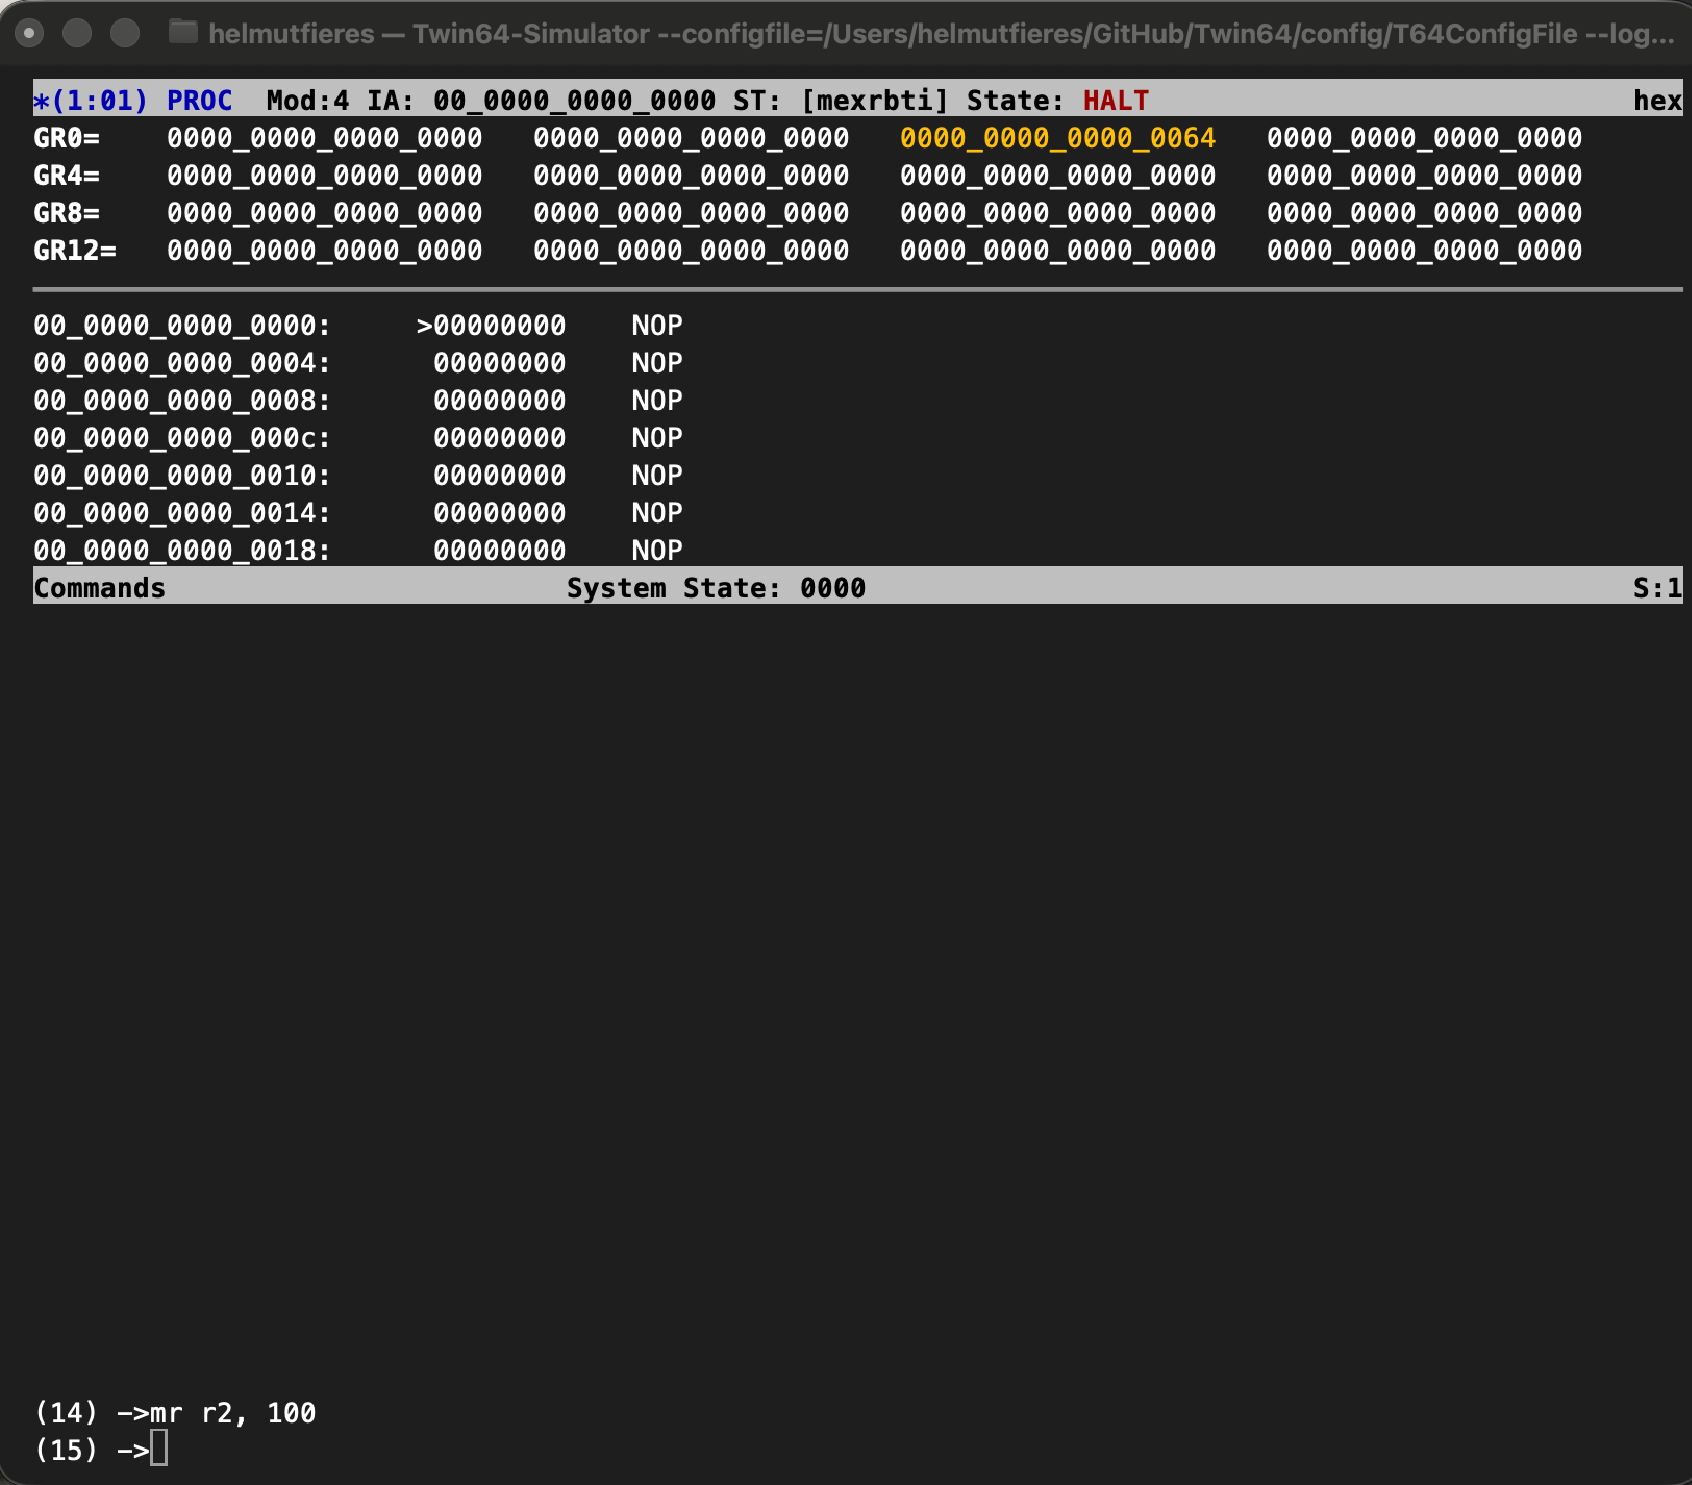
\includegraphics[width=16cm]{chapter-simulator-environment/SimWinProcReg.pdf}};
\end{tikzpicture}
\caption{Simulator CPU Window — General Registers}
\label{fig:simulator-cpu-window-greg}
\end{figure}

The window consist of two main parts. The first part shows the processor register set. This part can be toggled to show the general registers, ( default ), the control registers and a user visible subset of the control registers. The second pat depicts the actual code where the instruction address register points to. This area can be modified to show more than the default lines of 6 lines. A mark shows where exactly the current instruction address is located. Values modified are highlighted until the next command.

As with all simulator windows, multiple instances of the same window type may be created. In the case of the CPU window, all three view modes can be displayed simultaneously by creating multiple windows and toggling each one to the desired view.


%--------------------------------------------------------------------------------
\section*{TLB Window}
\addcontentsline{toc}{section}{TLB Window}

The TLB (Translation Lookaside Buffer) window displays the contents of the simulator global TLB module. The TLB accelerates virtual-to-physical address translation by caching recently used page table entries. The global TLB module is the TLB which all processors consult when in need for a translation.  The translation result is then kept in local TLB buffers on the processor module. Featuring a global TLB allows all memory commands and windows to use physical and virtual addresses without being dependent on which processor actually has a valid translation.

\begin{figure}[H]
\centering
\begin{tikzpicture}[x=1cm, y=1cm, scale=0.7, transform shape]
    \node[anchor=south west] (img) at (0, 0)
        {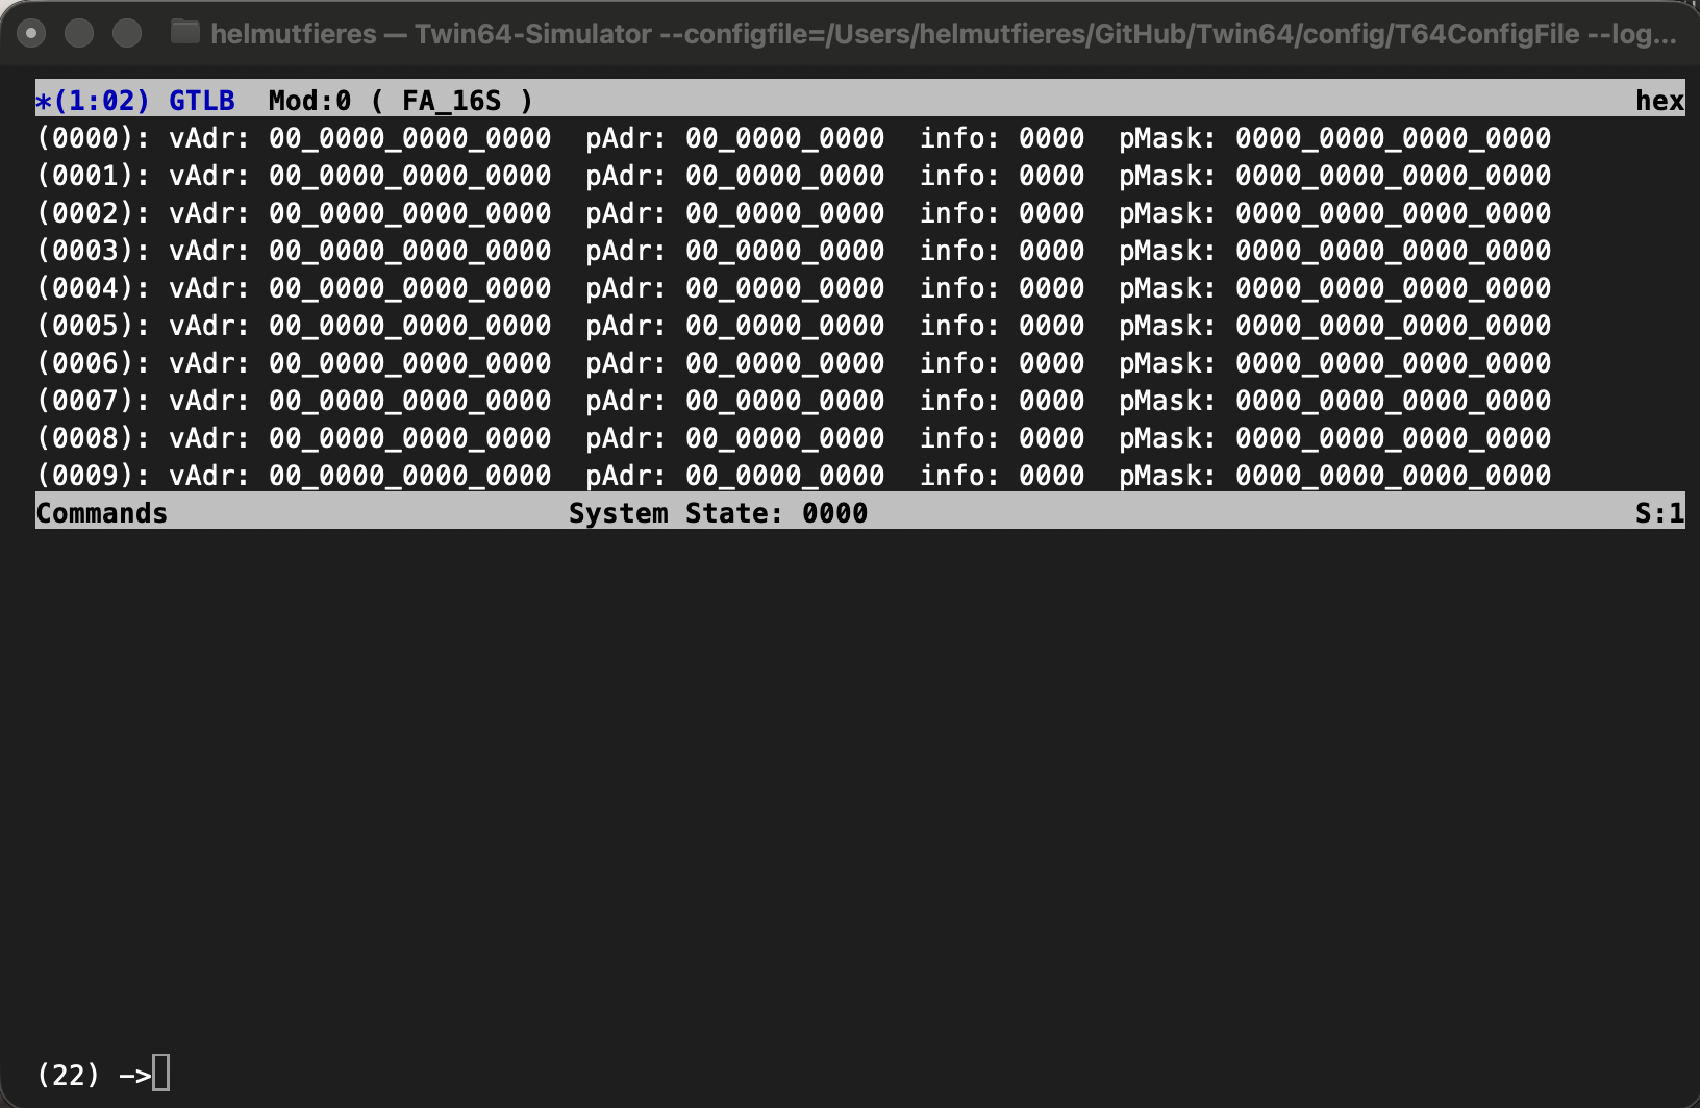
\includegraphics[width=16cm]{chapter-simulator-environment/SimWinTlb.pdf}};
\end{tikzpicture}
\caption{Simulator TLB Window}
\label{fig:simulator-tlb-window}
\end{figure}

The global TLB window displays the TLB entries line by line. Each entry includes the virtual page tag, the corresponding physical page number, and the associated tlbInfo. The final field is the tlb page mask when the TLB supports a variable page size. 

%--------------------------------------------------------------------------------
\section*{Memory Window}
\addcontentsline{toc}{section}{Memory Window}

The memory window displays the contents of physical or virtual memory. The banner line contains the window identifier, the memory module number, and the window's home address. This information allows the user to quickly identify the memory region being examined. 

\begin{figure}[H]
\centering
\begin{tikzpicture}[x=1cm, y=1cm, scale=0.7, transform shape]
    \node[anchor=south west] (img) at (0, 0)
        {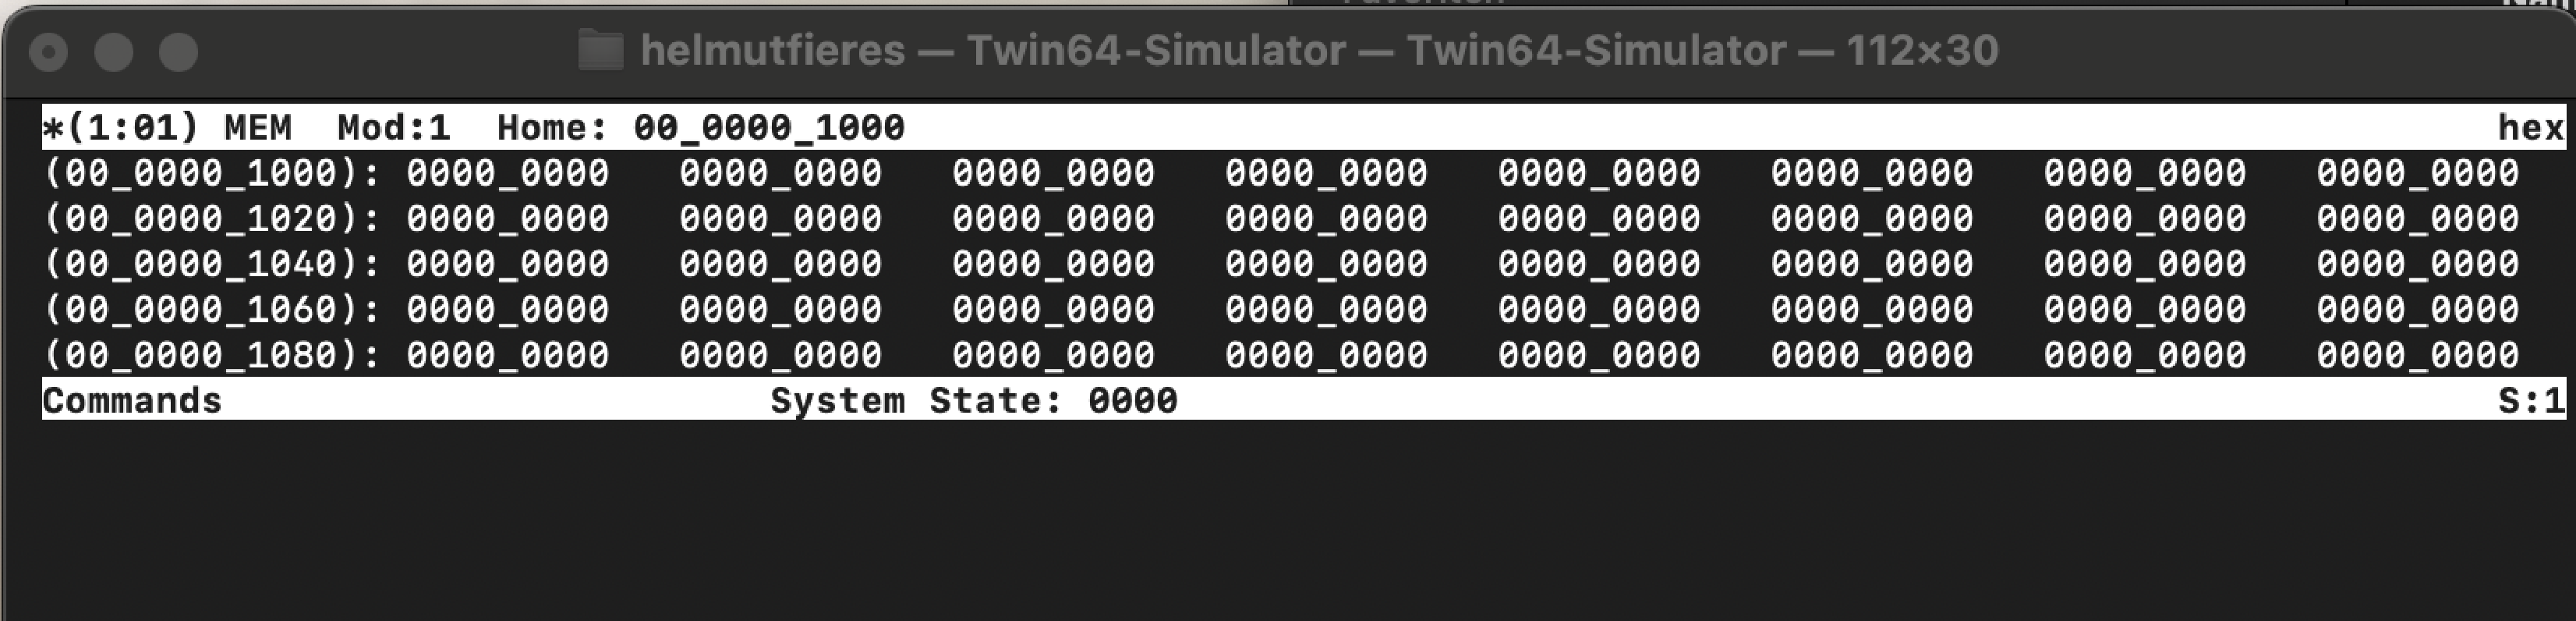
\includegraphics[width=16cm]{chapter-simulator-environment/SimWinMemHex32.pdf}};
\end{tikzpicture}
\caption{Simulator Memory Window — Hexadecimal (32-bit)}
\label{fig:simulator-mem-window-hex32}
\end{figure}

The memory window provides several display modes that allow memory data to be viewed in different formats, depending on the debugging task at hand. The window can be toggled between these modes while maintaining the same base address and line alignment.

In the 32-bit hexadecimal display mode, memory is shown as a sequence of 32-bit words formatted in hexadecimal notation. This view is useful for inspecting instruction streams and word-oriented data structures.

The 64-bit hexadecimal display mode presents memory as 64-bit quantities. This format is convenient for examining double-word data values and pointer-sized objects. In decimal mode, memory contents are displayed as signed decimal values. This view is intended primarily for examining numeric data produced or consumed by applications.

The ASCII display mode interprets memory bytes as printable characters. Non-printable bytes are shown using a placeholder representation. This mode is useful for inspecting strings, text buffers, and structured data with embedded character fields.

The code window toggle of a memory window displays the contents of memory in a disassembled form, allowing the user to examine instructions as human-readable assembly code. This window helps in debugging by showing the relationship between machine code in memory and its corresponding assembly instructions.

%--------------------------------------------------------------------------------
\section*{Text Window}
\addcontentsline{toc}{section}{Text Window}

The text window displays the contents of a text file. The banner line contains the window identifier, the memory or file module number, and the window's home address, allowing the user to quickly identify the source and location of the displayed text.

\begin{figure}[H]
\centering
\begin{tikzpicture}[x=1cm, y=1cm, scale=0.7, transform shape]
    \node[anchor=south west] (img) at (0, 0)
        {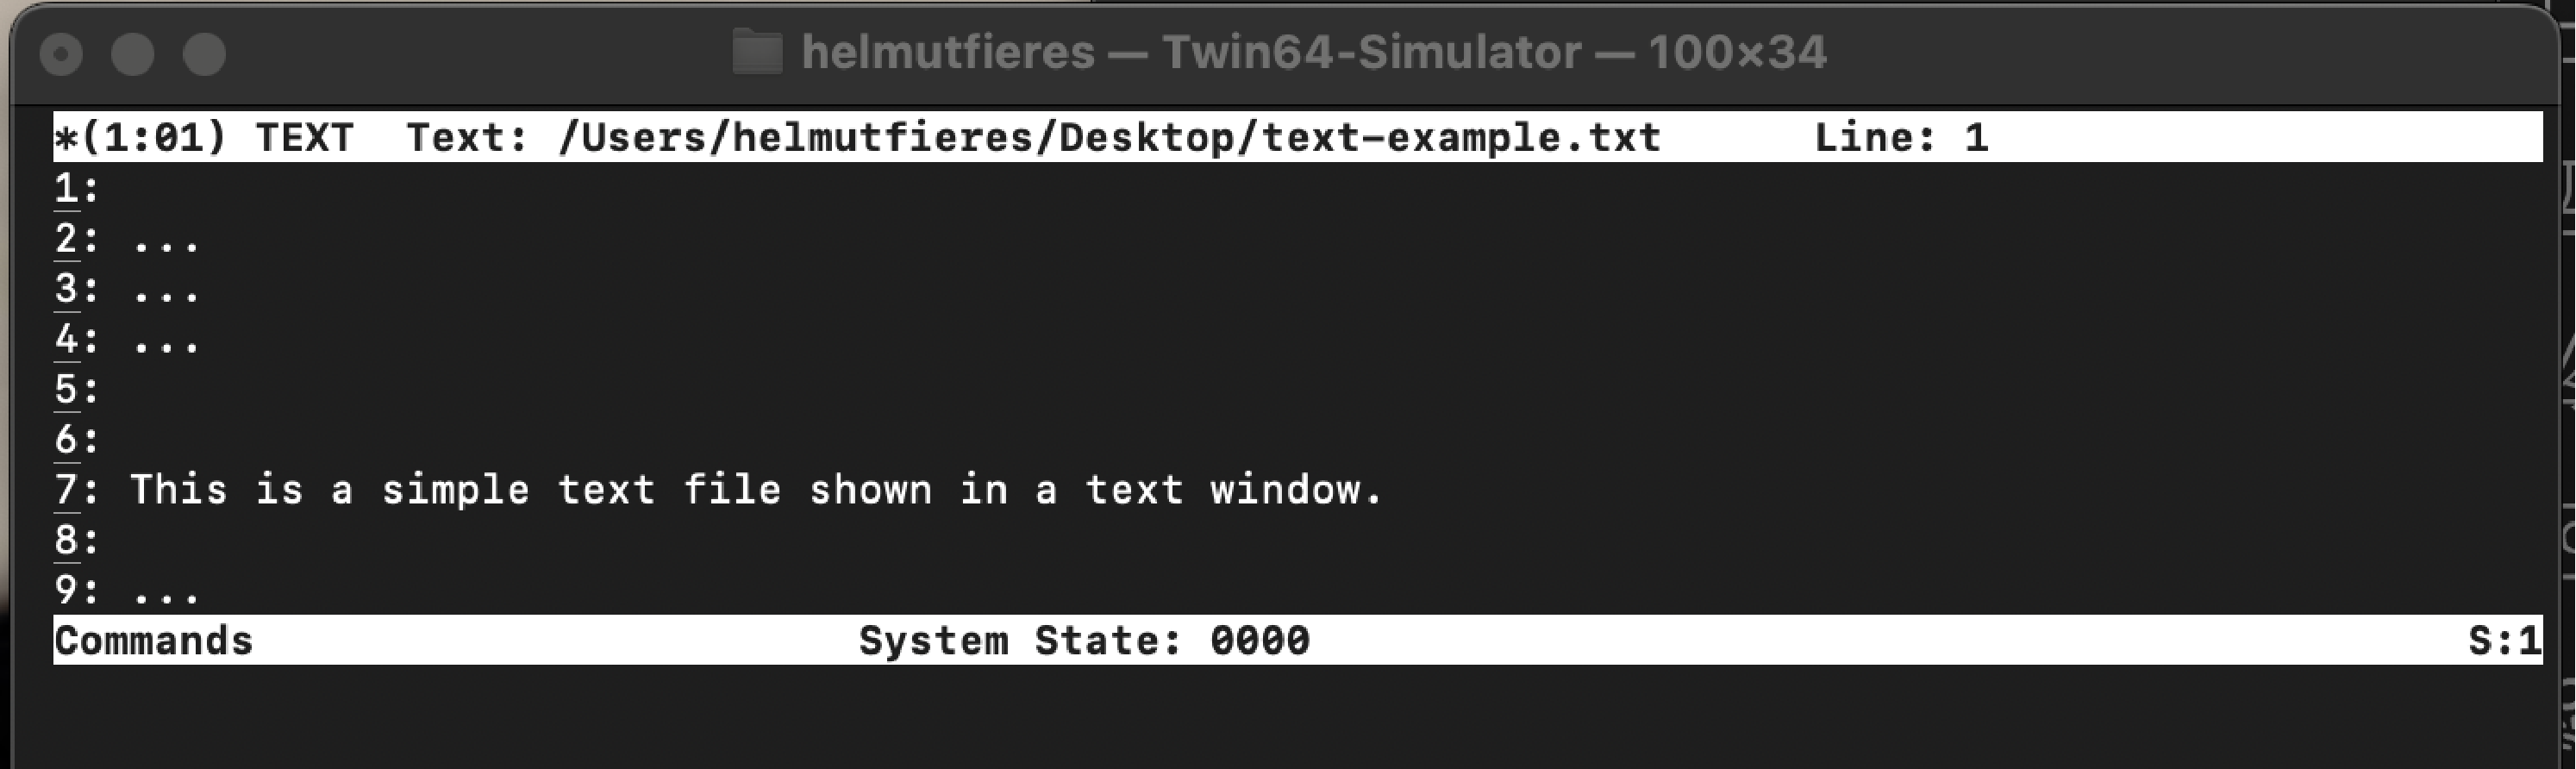
\includegraphics[width=16cm]{chapter-simulator-environment/SimWinText.pdf}};
\end{tikzpicture}
\caption{Simulator Text Window}
\label{fig:simulator-text-window}
\end{figure}

The text window displays the content line by line. It preserves formatting such as line breaks and spaces, making it suitable for inspecting textual data exactly as it would appear in a file or console output.
